% Chapter 5
\chapter{Implémentation, simulation et résultats}

\label{Chapter5}
Au cours de ce chapitre nous allons présenter l'implémentation et le test de notre système dans un réseau SDN qu'on va simuler. On commence par voir l'environnement de travail, les outils de simulation utilisés, pour passer ainsi à la phase des tests, qui est divisée en deux: premièrement nous allons tester notre programme sur un jeu de données qu'on verra varier pour calculer les différentes métriques citées dans la section \ref{evaluation}, ensuite on testera notre système dans un réseau SDN simulé sur plusieurs scénarios, d'attaques et de flux normaux, pour étudier son comportement dans un réseau en production.

\section{Environnement de travail}
Cette partie décrit l'environnement SDN dans lequel on a développé notre solution en présentant le contrôleur SDN choisi et l'outil de simulation du réseau utilisé.

\subsection{Contrôleur SDN}
Parmi les différents contrôleurs SDN qui existent, nous avons opté pour travailler avec \textbf{Ryu}[\cite{4}] vu la simplicité d'utilisation qui offre, en plus il est basé sur \textit{Python} et supporte la majorité des versions d’OpenFlow. \\\\
Ryu est un contrôleur de réseau défini par logiciel (SDN) conçu pour augmenter l’agilité du réseau en le rendant facile à gérer et adapte la façon dont le trafic est traité. Il fournit des composants logiciels, avec des interfaces de programme d’application (API) bien définies, qui rendent facile pour les développeurs de créer de nouvelles applications de gestion et de contrôle du réseau. Cette approche par composants aide les organisations à personnaliser leurs déploiements pour répondre à leurs besoins spécifiques; les développeurs peuvent rapidement et facilement modifier les composants existants ou mettre en œuvre leurs propres pour s’assurer que le réseau sous-jacent peut répondre aux demandes changeantes de leurs applications.\\

\noindent Pour télécharger et installer Ryu sur une machine UBUNTU:
\begin{verbatim}
% git clone git://github.com/faucetsdn/ryu.git
% cd ryu
% pip install .
\end{verbatim}


\subsection{Simulation du réseau SDN}
Afin de pouvoir déployer notre système dans un environnement SDN pour le tester, on est obligé de simuler un réseau SDN réel avec tous ces équipements, contrôleurs SDN, commutateurs, hôtes, liens physiques. Ceci est possible à l'aide d'un émulateur réseau. Il en existe beaucoup d'émulateurs réseau, celui qui nous convient dans notre travail est \textit{Mininet}[\cite{28}].

\subsubsection{Mininet}
Mininet est un émulateur de réseau qui crée un réseau d’hôtes virtuel, de commutateurs, de contrôleurs et de liens. Les hôtes Mininet exécutent le système \textit{Linux} standard, ce qui donne la possibilité d'exécuter des programmes au niveau des hôtes. Les commutateurs prennent en charge Openflow pour un routage personnalisé hautement flexible.

\noindent Mininet est vaguement recommendé car:\\
\begin{itemize}
\item[-] Est rapide, démarrer un réseau simple ne prend que quelques secondes.\\
\item[-] Vous pouvez créer des topologies personnalisées : un commutateur unique, de plus grandes topologies de type Internet, un centre de données, ou toute autre chose.\\
\item[-] Vous pouvez personnaliser le transfert de paquets : les commutateurs de Mininet sont programmables à l’aide du protocole Openflow.\\
\item[-] Comprend une interface de lines de commande \textbf{CLI} pour le débogage ou l’exécution de tests sur réseau.\\
\end{itemize}

\noindent Pour installer mininet sur une machine UBUNTU:
\begin{verbatim}
% sudo apt install mininet
\end{verbatim}
Ou bien: 
\begin{verbatim}
% git clone git://github.com/mininet/mininet
% mininet/util/install.sh
\end{verbatim}

\subsubsection{Simulation d'un simple réseau SDN}
Ci-dessous un exemple sur comment lancer la simulation d'un simple réseau SDN avec un contrôleur, un switch OpenFlow et deux hôtes.\\

\noindent 1- Lancer le contôleur Ryu:
\begin{verbatim}
% ryu-manager ryu_controller.py 
\end{verbatim}
2- Créer la topologie avec mininet:
\begin{verbatim}
% sudo mn --controller remote --topo single,2 --switch ovs --mac
\end{verbatim}

\begin{tabular}{m {13cm}}
\hline
\textbf{\textit{Terminal}} - topologie créée par mininet\\
\hline
\begin{verbatim}
*** Creating network
*** Adding controller
Connecting to remote controller at 127.0.0.1:6653
*** Adding hosts:
h1 h2 
*** Adding switches:
s1 
*** Adding links:
(h1, s1) (h2, s1) 
*** Configuring hosts
h1 h2 
*** Starting controller
c0 
*** Starting 1 switches
s1 ...
*** Starting CLI:
mininet> 
\end{verbatim}\\
\hline
\end{tabular}

\section{Langage et Librairies utilisées}

\subsection{Python}
Python est un langage de programmation très puissant et adaptable à tout type d’utilisation grâce à ces bibliothèques spécialisées, utilisé particulièrement comme un langage de script. Il est trop utilisé dans la programmation réseau et spécialement dans les réseaux SDN.

\subsection{Scikit-learn}
Scikit-learn est une bibliothèque libre Python destinée à l'apprentissage automatique. Elle est développée par de nombreux contributeurs2 notamment dans le monde académique par des instituts français d'enseignement supérieur et de recherche comme Inria3. Elle comprend notamment des fonctions pour estimer des forêts aléatoires, des régressions logistiques, des algorithmes de classification, et les machines à vecteurs de support. Elle est conçue pour s'harmoniser avec d'autres bibliothèques libres Python, notamment NumPy et SciPy.[\cite{29}] 

\subsection{Pandas}
Pandas est une bibliothèque écrite pour le langage de programmation Python permettant la manipulation et l'analyse des données. Elle propose en particulier des structures de données et des opérations de manipulation de tableaux numériques et de séries temporelles.\\
\noindent Les principales structures de données sont les séries (pour stocker des données selon une dimension - grandeur en fonction d'un index), les DataFrames (pour stocker des données selon 2 dimensions - lignes et colonnes), les Panels (pour représenter des données selon 3 dimensions, les Panels4D ou les DataFrames avec des index hiérarchiques aussi nommés MultiIndex (pour représenter des données selon plus de 3 dimensions). [\cite{30}]

\subsection{Argus}
Argus[\cite{31}] est le premier système de flux réseau, développé par Carter Bullard au début des années 1980 à Georgia Tech. La technologie de flux réseau est devenue un élément essentiel de la cybersécurité moderne et Argus est utilisé dans certains des réseaux les plus importants du monde. Le système Argus tente de résoudre un grand nombre de problèmes liés aux données de flux réseau : échelle, performance, applicabilité, confidentialité et utilité.\\
Nous avons utilisé Argus pour calculer les propriétés des flux qui circulent dans notre réseau SDN, parmi ses propriétés: durée de flux, nombre de paquet par seconde, nombre total de paquets, taille du paquet,...etc.

\section{Réalisation du module F-Clustering}
On rapelle que ce module est modèle intélligent qui utilise une approche de clustering pout la détection des attaques. Dans la section \ref{F-Clustering}, nous avons décrits les étapes à suivre pour construire notre modèle de clustering qui sont accomplies à l'aide des deux programmes pythons, "Preprocessos.py" et "Cluster.py".
\begin{algorithm}[H]
\begin{verbatim}

1- def preprocessor (df):
 
2- 	df = cleanDataFrame(df) # Data laundry
3- 	df = balanceDataFrame(df) 
4- 	df = scaleDataFrame(df)

5- 	return df
\end{verbatim}
\caption{Preprocessor.py}
\end{algorithm}

\begin{algorithm}[H]
\begin{verbatim}

1- from Preprocessor.py import preprocessor 
2- from sklearn.cluster import KMeans

4- df = pd.read_csv('TFTP.csv')
5- newDF = preprocessor(df)

6- centers = calculateCenters(newDF) #returns 2 elements array
7- F_Clustering = KMeans(n_clusters=2, init=centers).fit(newDF) 

\end{verbatim}
\caption{Cluster.py}
\end{algorithm}

\section{Évaluation et test des performances}
Dans cette partie, nous allons entamer l'étape du processus KDD, qui est l'évaluation du modèle. Les résulatats des test de performance de montre modèle étaient les suivants, il est à noter que le jeu de données de test est le dataset "TFTP" aprés le prétraitement et qui contient 1.315.348 lignes.

\begin{table}[h]
	\begin{center}
		\begin{tabular}{  | m{2.5cm} | m{2.5cm} | m{2.5cm} || m{2cm} | }
			\hline
			  & Attaques & Bénins & Total\\
			\hline
			Attaques & 657674 & 0 & 657674\\
			\hline
			Bénins & 8887 & 648787 & 657674\\
			\hline
		\end{tabular}
		\caption{Matrice de confusion}
	\end{center}
	\label{table:NIDS_Evaluation}
\end{table}

\begin{table}[h]
	\begin{center}
		\begin{tabular}{  | c | c | c | c | c | }
			\hline
			\rowcolor[rgb]{0.85,0.85,0.85}
			 Exactitude & Précision & Rappel & F1-Measure & Taux de fausses alertes\\
			\hline
			99.3\% & 98.6\% & 100\% & 99.3\% & 1.3\%\\
			\hline
		\end{tabular}
		\caption{Mesures de performance }
	\end{center}
	\label{table:F_Clustering_Evaluation}
\end{table}

Nous remarquons que les résultats sont trés satisfaisants. L'élément clé qui nous a permis d'avoir tel résultats c'est les prétraitements faits sur le dataset, plus spécialement l'opération de normalisation et l'opération blancement. Pour montrer leur impact  sur les performance du modèle, nous allons faire une petite experience, où nous allons anuller une opération de prétraitemnt à la fois, soit la normalisation, soit le balancement et calculer ensuite les mesures de performance du modèle.\\

Les résulatats obtenus sont dans le tableau suivant:
\begin{table}[h]
	\begin{center}
		\begin{tabular}{  | c | c | c | c | }
			\hline
			 Opération(s) effecutée(s) & Exactitude & Rappel & F1-Measure \\
			\hline
			\hline
			Aucune & 25.4\% & 24.4\% & 39.2\% \\
			\hline
			Normalistion seulement & 29.6\% & 27.6\% & 43.2\% \\
			\hline
			Balancement seulement & 71.5\% & 43.8\% & 60.6\% \\
			\hline
			\rowcolor[rgb]{0.75,0.75,0.75}
			Balancement + Normalisation & 99.3\% & 100\% & 99.3\% \\
			\hline
		\end{tabular}
		\caption{Impact des prétraitements sur les performance}
	\end{center}
	\label{table:compare}
\end{table}

\begin{figure}[h]
\centering
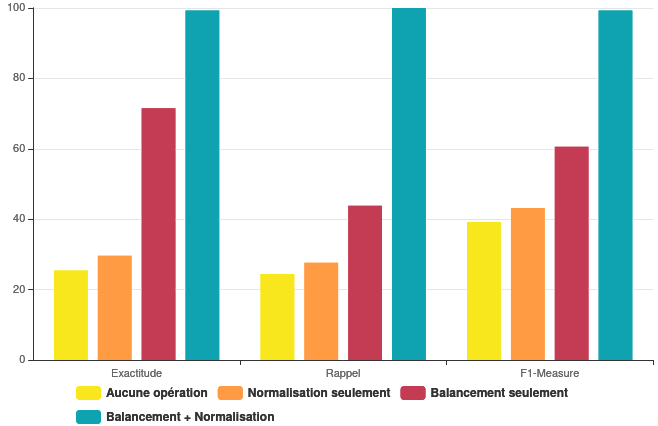
\includegraphics[width=0.8\textwidth]{Figures/performances}
\decoRule
\caption{Comparaison entre les résultats obtenus selon l'opération de prétraitement effectuée}
\label{fig:rDoS}
\end{figure} 
